\myparagraph{Purpose}
As we have the possibilty in \textit{Track4Run} for a runner to be able to enrol in a \textit{Run}, the system must also be able to manage the decision of a runner to delete his/her enrolment.

\myparagraph{Scenario}
Giulia is enrolled in the annual \textit{Run} of her neighborhood. The enrolment management was made through \textit{Track4Run} application. Unfortunately for the day of the \textit{Run} Giulia will be in Florence for an important work meeting.
When Giulia received the meeting mail she took her phone, she opened \textit{Track4Run} app and she clicked on "\textit{Enrolled Run}" button.
The only row in the table was the annual \textit{Run}, Giulia clicked on it and then clicked on "\textit{Delete Enrolment}" button.
After that Giulia received a confirmation e-mail.

\myparagraph{Use Case}
The \textit{Delete an Enrolment in a Run} use case is analyzed in Table \ref{table:deleteEnrolmentTable}.

\myparagraph{Activity Diagram}
The \textit{Delete an Enrolment in a Run} activity diagram is shown in Figure \ref{img:deleteEnrolmentActrivityDiagram}.

\myparagraph{Mockup}
The \textit{Delete an Enrolment in a Run} mockup is shown in Figure \ref{img:deleteEnrolmentMockup}.

\myparagraph{Functional requirements}
\begin{enumerate}
  \item The system must not show \textit{Run}, in \textit{Enrolled Run} section, in which a \textbf{Runner} is not enrolled;
  \item The system must let the \textbf{Runner} delete his/her enrolment in a \textit{Run} at anytime;
  \item The system must let the \textbf{Runner} leave the elimination process at anytime.
\end{enumerate}

\begin{center}[H]
\begin{table}
\begin{tabular}{ | l | p{0.75\linewidth} | }
  \hline
    Actor & \textbf{Runner} \\ \hline
    Goal & \textbf{[G.13]} \\ \hline
    Input Condition & A \textbf{Runner} wants to delete an enrolment in a \textit{Run} \\ \hline
    Event Flow & \begin{minipage}[t]{0.7\textwidth}
      \begin{enumerate}
        \item The \textbf{Runner} opens \textit{Track4Run} service through mobile application and he/she logs in;
        \item The \textbf{Runner} clicks on the "\textit{Enrolled Run}" button;
        \item The \textbf{Runner} looks for a \textit{Run} through the search bar or looking to the proposed ones;
        \item The \textbf{Runner} clicks on the \textit{Run} in which he/she wants to delete the enrolment;
        \item The \textbf{Runner} clicks on the "\textit{Delete Enrolment}" button.
      \end{enumerate}
    \smallskip
  \end{minipage} \\ \hline
  Output Condition & The system deletes the enrolment of the \textbf{Runner} and it notifies him/her with a confirmation e-mail. \\ \hline
  Exceptions & \begin{minipage}[t]{0.7\textwidth}
    \begin{itemize}
      \smallskip
      \item If the \textbf{Runner} looks for a \textit{Run} that is not present in the system, the system notifies the \textbf{Runner} with a warning message;
      \item If the \textbf{Runner} decides to leave the elimination process this one is aborted.
    \end{itemize}
    \smallskip
  \end{minipage}  \\ \hline
\end{tabular}
\caption{\textit{Delete an Enrolment in a Run} use case}
\label{table:deleteEnrolmentTable}
\end{table}
\end{center}

\begin{figure}[H]
\begin{center}
  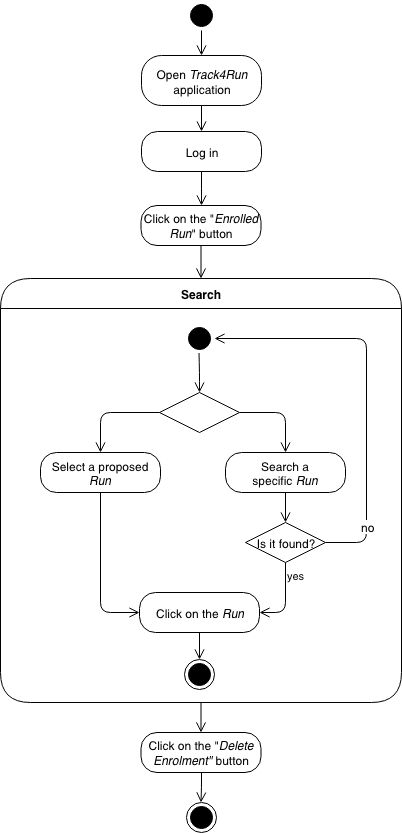
\includegraphics[height=0.6\paperheight]{img/activity/DeleteEnrolment.png}
  \hspace{0.05\linewidth}
  \centering
  \caption{\textit{Delete an Enrolment in a Run} activity diagram from user's point of view}
  \label{img:deleteEnrolmentActrivityDiagram}
\end{center}
\end{figure}

\begin{figure}[H]
\begin{center}
  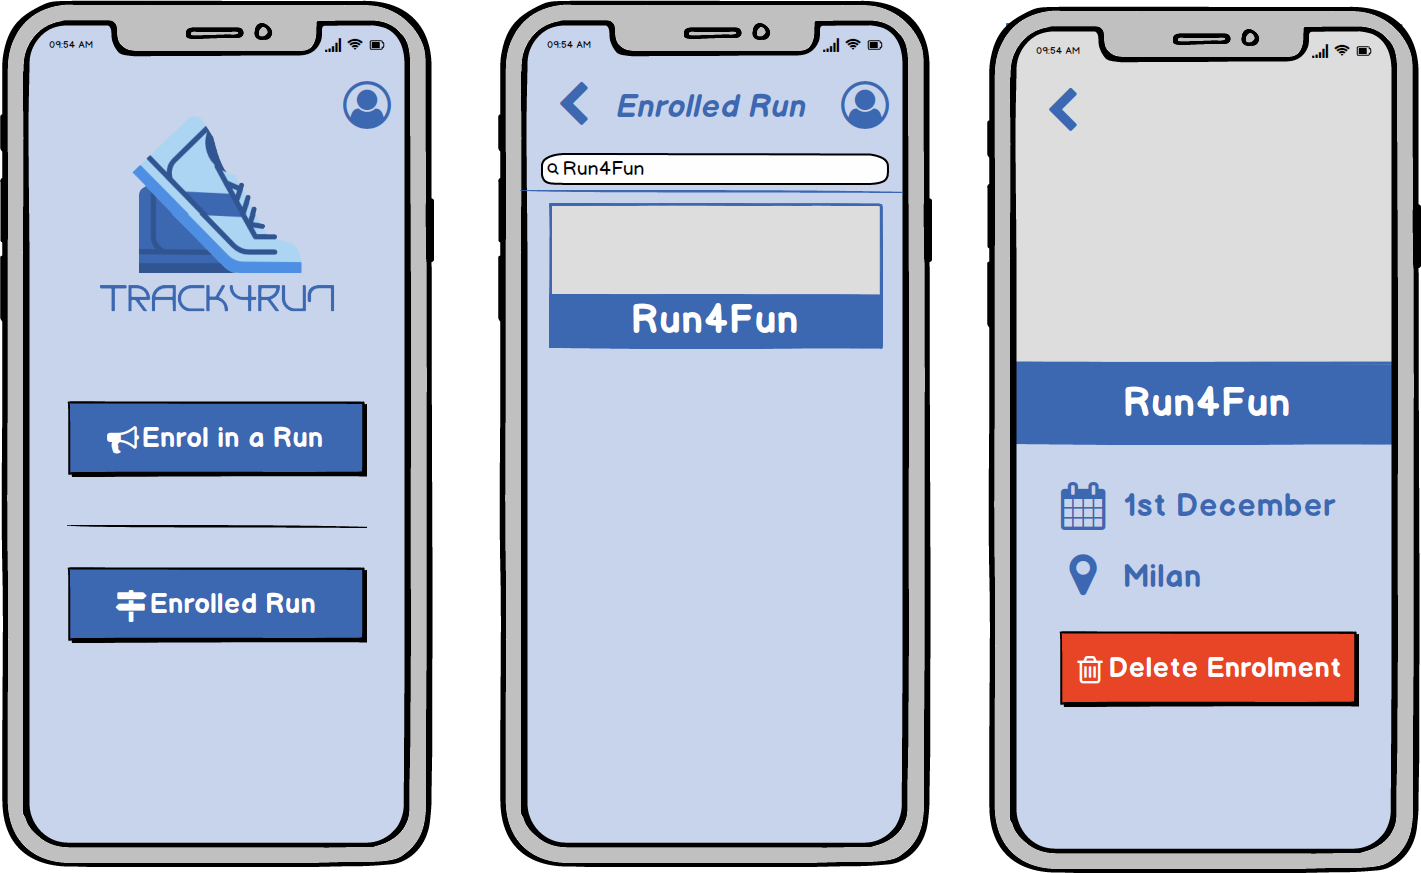
\includegraphics[width=\textwidth]{img/mockup/DeleteEnrolment.png}
  \hspace{0.05\linewidth}
  \centering
  \caption{\textit{Delete an Enrolment in a Run} mockup}
  \label{img:deleteEnrolmentMockup}
\end{center}
\end{figure}
